\subsection{Linear Momentum}
We mentioned linear momentum a bit in our discussion about forces, defining the product of an object's mass and velocity to be this quantity, as follows: 
\[
	\vec P = m \vec v
\]
where $\vec P$ stands for linear momentum. This is a vector quantity and has the same direction as the velocity and units of kg $\cdot$ m/s = N $\cdot$ s. 
\subsubsection{Impulse-Momentum Theorem}
Impulse is something that often comes up with discussions of linear momentum, and it would seem at first like a completely separate quantity. The impulse delivered to an object $\vec J$, in terms of the net force $\vec F$ on it over a time interval $[t_1, t_2]$ is defined to be the following: 
\[
	\vec J = \int_{t_1}^{t_2} \vec F \, dt
\]
Recall we can write the force $\vec F = \dv{\vec P}{t} = m \vec a$, so this becomes:
\[
	\vec J = \int_{t_1}^{t_2} \dv{\vec P}{t} \, dt = \vec P(t_2) - \vec P(t_1) = \Delta \vec P
\]
So, impulse is nothing terribly special - it's equal to the change in linear momentum delivered to a particle. This is also true in general for systems of particles - the total impulse delivered to a system is equal to the change in the total linear momentum of the system. This is the Impulse-Momentum Theorem, relating impulse to linear momentum. \\
We can go one step further. Notice that the average force on an object $\vec F_{av}$ is
\[
	\vec F_{av} = \frac{\Delta \vec P}{\Delta t}
\]
so the impulse delivered to the system over a time $\Delta t$ is just 
\[
	\vec J = \vec F_{av} \Delta t
\]
\subsubsection{Center of Mass}
The center of mass is a tool we need to use in order to use momentum effectively. From up until this point we have been operating under the assumption that objects effectively behave like a point particle. This really isn't true - after all, something like a baton when thrown into the air spins, and the motion of the end of the baton does not follow a perfect parabolic path as kinematics would have us believe. However, we know for certain that one point in the baton system follows this parabolic trajectory, being the center of mass. \\
First, let's just define the center of mass of a system of particles. Say with respect to some reference point these particles have position vectors $\vec r_i$, where $i$ goes from $1$ to however many particles there are. If each particle also has a mass $m_i$, and the mass of all of the particles is $M$, then the position of the center of mass $\vec r_{cm}$ is: 
\[
	\vec r_{cm} = \frac{1}{M} \sum_i m_i\vec r_i
\]
Essentially, this is a weighted average of the positions of each particle with respect to the mass. Since the masses are all scalars, we can take derivatives to find the velocity and acceleration of the center of mass, showing that these can also be found by taking the mass-weighted average of all the velocities and accelerations, respectively, of the particles. 
\[
	\vec v_{cm} = \dv{\vec r_{cm}}{t} = \dv{}{t} \frac{1}{M} \sum_i m_i \vec r_i = \frac{1}{M} \sum_i m_i \dv{\vec r_i}{t} = \frac{1}{M} \sum_i m_i \vec v_i
\]
\[
	\vec a_{cm} = \dv{\vec v_{cm}}{t} = \dv{}{t} \frac{1}{M} \sum_i m_i \vec v_i = \frac{1}{M} \sum_i m_i \dv{\vec v_i}{t} = \frac{1}{M} \sum_i m_i \vec a_i
\]
So how to find the center of mass? For a discrete collection of particles, the calculations are fairly straightforward - one just projects into components, and uses the same mass-weighted average to find the $x$-, $y$-, etc. components of the center of mass. Putting it all together with appropriate unit vectors gives the correct position vector. \\
For continuous distributions of mass, we have to be a bit more clever. If we let the mass of each little particle/subsection in a larger object go to zero as we divide it up into smaller and smaller pieces, then we can compute the desired sum as an integral by summing together all the appropriate pieces. This gives us:
\[
	\vec r_{cm} = \frac{1}{M} \int \vec r \, dm
\]
where $\vec r$ is the position vector of each infinitesimally small mass portion $dm$. 
Usually, when computing the center of mass for continuous distributions we define a density function $\lambda$, which represents mass per unit length. (AP Physics doesn't require being able to compute the center of mass for two/three/higher dimensional objects.) As a basic example, a rod with uniform density and mass $M$ and length $L$ has its center of mass in the middle of the rod, by symmetry. As a more nontrivial example, consider a semicircle with radius $R$ and uniform density (mass per unit length) $\lambda$.
\begin{center}
	\begin{asy}
		import olympiad;
		pair O, P, X;
        size(8cm);
		O = (0,0);
		dot(O);
		draw(arc(O, 1, 0, 180));
		real dtheta = 8;
		real angle = 40;
		X = dir(angle);
		P = dir(angle+dtheta);
		draw(O--P, linetype("8 8"));
		draw(O--X, linetype("8 8"));
		real vertoffset = -0.1;
		draw((0, vertoffset)--(-1, vertoffset), linetype("8 8"), arrow=Arrows());
        draw(dir(180)--dir(0), linetype("4 4"));
        draw(arc(O, 0.8, angle, angle+dtheta), arrow=Arrows());
        dot(2*dir(90)/pi);
        
        label("$\theta$", 0.15*dir(angle/2), dir(angle/2));
        label("$ds$", dir(angle+dtheta/2), dir(angle+dtheta/2));
        label("$R$", (-0.5, 1.2*vertoffset), dir(270));
        label("$d\theta$", 0.7*dir(angle-dtheta), dir(angle-dtheta));
        label("COM", 2*dir(90)/pi, NW);
	\end{asy}
\end{center}
Because the semicircle is uniform, we know that $\lambda = \frac{M}{\pi R}$, but we're not going to plug it into our expressions until the end. Let the $x$-axis be the diameter of the semicircle, and the $y$-axis the line through the center perpendicular to it. From here, we're going to use polar coordinates. \\
The vector $\vec r$ for all points on the semicircle is $R \cos \theta \, \hat x + R \sin \theta \, \hat y$, as $\theta$ ranges from $0$ to $\pi$. Now, we have to express $dm$ in terms of $\theta$. Note since each small piece is a small arc of the semicircle, $dm = \lambda \, ds$, where $ds$ is a small arc. We know that $ds = R \, d\theta$, so at the end of the day we have $dm = \lambda R \, d\theta$. Now, we can integrate and evaluate: 
\begin{align*}
	\vec r_{cm} &= \frac{1}{M} \int \vec r \, dm\\
	&= \frac{1}{M} \int_0^\pi \lambda R (R \cos \theta \, \hat x + R \sin \theta \, \hat y) \, d\theta \\
	&= \frac{\lambda R^2}{M} \int_0^\pi \cos \theta \, \hat x + \sin \theta \, \hat y \, d\theta \\
	&= \frac{\lambda R^2}{M} \left( \int_0^\pi \cos \theta \, d\theta \, \hat x + \int_0^\pi \sin \theta \, d\theta \, \hat y \right)\\
	&= \frac{\lambda R^2}{M} \left( \sin \theta \Big |_0^\pi \hat x - \cos \theta \Big|_0^\pi \, \hat y \right)\\
	&= \frac{2}{\pi}R \, \hat y
\end{align*}
Notice that we could have simplified our calculations a little bit, since we would have only needed to consider the $y$-component because the $x$-component would've come out to be $0$ by symmetry. This result is also a bit strange, in that the center of mass doesn't actually lie on the actual body of mass, but the result is in fact correct. A similar procedure to what we've done here can be applied to other continuous mass distributions and even non-uniform bodies given the density function $\lambda$.

\subsubsection{Conservation of Linear Momentum}
The center of mass of a system of particles may seem clunky to use or not quite connected to what we've done so far, but we can connect it to what we've established so far about dynamics. \\
The sum of all the forces on all the particles in a system is the following, by Newton's Second Law: 
\[
	\sum_i \vec F_i = \sum_i m_i \vec a_i 
\]
We can divide up these forces into those that are external to the system, and those that are internal to the system and multiply/divide on the right-hand side by the total mass $M$: 
\[
	\vec F_{net}^{int} + \vec F_{net}^{ext} = M \frac{1}{M}\sum_i m_i \vec a_i 
\]
Notice, however, that by Newton's Third Law, the internal forces are all part of action-reaction pairs, which all sum to zero. Therefore, we can eliminate that term. Furthermore, we can substitute in the acceleration of the center of mass $\vec a_{cm}$:
\[
	\vec F_{net}^{ext} = M \vec a_{cm} = \dv{\vec P_{sys}}{t}
\]
This is a more general form of Newton's Second Law, but for a system of particles rather than just a singular point particle. Similarly, by integrating this in the same way as before, the total linear momentum of the system $\vec P_{tot}$ is:
\[
	\vec P_{tot} = M \vec v_{cm}
\]
What if the sum of the external forces on a system is zero? Then the linear momentum of the system $\vec P_{tot}$ is some constant. To be clear: 
\begin{mdframed}[frametitle=Conservation of Linear Momentum]
For a system with no external forces, linear momentum is conserved - the amount of linear momentum in the system remains constant and is not changed by the internal motion/dynamics of the system.
\end{mdframed}
\subsubsection{Rockets}
We're going to apply concepts of linear momentum to derive the rocket equation in one dimension. (This isn't part of the AP course, but it might show up on an exam.) In the most abstract sense, rockets shoot mass out their end to propel themselves forward, which usually takes the form of fuel (but Dr. Dell suggested using a cuter power source, such as having gerbils jump off the end).\\
\begin{center}
	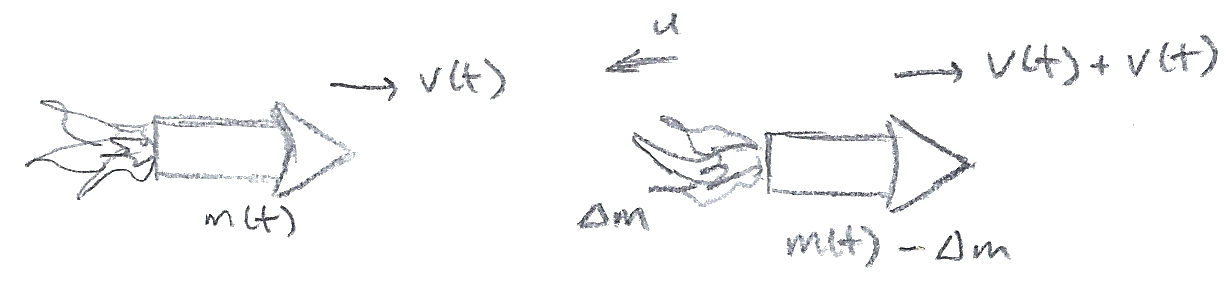
\includegraphics[width=0.5\textwidth]{images/mechintro/rockets.png}\\
\end{center}
To set this up, let $m(t)$ be the mass of the rocket as a function of time, $v(t)$ be the velocity (in one dimension, for simplicity) and $u$ be the exhaust velocity, or how fast the mass being shot out the back end is going. \\
Since we're assuming no external forces are acting on the system, we can apply conservation of linear momentum. At some time $t$, we know the magnitude of the momentum of the rocket, $P^{tot}$:
\[
	P^{tot}_i = m(t) v(t) 
\]
Now, after a time $\Delta t$, we know the rocket has changed by a mass $\Delta m$ (which is negative) and increased its speed by $\Delta v$. Relative to the rocket, the exhaust is being jettisoned backwards at a velocity of $-u$, but relative to the reference frame, since the rocket is moving at a velocity of $v(t) + \Delta v$, the exhaust is moving at a velocity $v(t) + \Delta v - u$. From this, we can calculate the magnitude of the total linear momentum after a small time interval:
\[
	P^{tot}_f = (m(t) + \Delta m)(v(t) + \Delta v) - \Delta m (v(t) + \Delta v - u)
\]
This looks a bit messy, but we can condense it to the following: 
\[
	P^{tot}_f = m(t)v(t) + m(t) \Delta v + \Delta m u 
\]
By conservation of linear momentum, $P^{tot}_i = P^{tot}_f$, so canceling $m(t)v(t)$ we have that:
\[
	m(t) \Delta v = - \Delta m u
\]
One final step: as the length of the time interval we observe $\Delta t$ goes to $0$, we want to consider the rate of change of the velocity and mass, so we will reformulate this in terms of derivatives:
\[
	m(t) \dv{v}{t} = - \dv{m}{t} u
\]
This is the rocket equation. The term on the right-hand side is defined as the thrust of the rocket. However, if we'd like to know an actual function that models the motion of the rocket, this isn't quite enough. We're going to solve our first differential equation to find the velocity of the rocket and its relation to the mass of the rocket over time. \\
Let's rearrange this as follows: 
\[
	\frac{1}{u} \dv{v}{t} = - \frac{1}{m(t)} \dv{m}{t} 
\]
Let's integrate both sides with respect to time from time $t=0$ to some arbitrary time $t$:
\[
	\int_0^t \frac{1}{u} \dv{v}{t} \, dt = - \int_0^t \frac{1}{m(t)} \dv{m}{t} \, dt 
\]
\[
	\int_0^t \dv{}{t}\left(\frac{v}{u}\right) \, dt = - \int_0^t \dv{}{t} \left(\ln m(t) \right) \, dt
\]
\[
	\frac{v(t)}{u} - \frac{v_0}{u} = \ln m_0 - \ln m(t) 
\]
To simplify even further, let's just assume the rocket starts from rest, so we end up with a final result of:
\[
	v(t) = u \ln \frac{m_0}{m(t)}
\]
where $m_0$ is the initial mass of the rocket. \\
A little bit of fiddling with this reveals why rockets have to carry so much fuel: in order to maximize the velocity rockets have to be able to shoot out fuel at top speeds, and burn up a lot of their mass in order to get to fast enough speeds to escape Earth's gravity. \\
A small sidenote - letting $u$ be arbitrarily large creates problems not only practically, but also in theory: as $u$ approaches the speed of light, this model will give us velocities that are way over that speed - but the speed of light turns out to be a "speed limit" on the universe - nothing can travel faster than that. So there's something wrong with one of our assumptions somewhere! It turns out the correct expression for momentum isn't what we think it is at large speeds, but works for small speeds well enough - we'll discuss this if we talk about special relativity. 
\subsubsection{Summary and Problems}
Linear momentum is a good quantity to keep track of, especially when no outside forces are acting on the system like during a collision or explosion, in order to see how objects in the system move. We also learned how to calculate use the center of mass of an object to properly see how forces can impact the trajectory of the object, even if the situation is too computationally intensive to know the full motion of the block. \\

\noindent \textbf{Problems}\\
1. (2 $\bigstar$) A bullet with mass $m_1$ moving directly upward with speed $v_i$ strikes and passes through the center of mass of a block with mass $m_2$ which is initially at rest. The bullet emerges from the block moving directly upward and has slowed to a speed $v_f$. Show that the maximum height $h$ that the block rises above its initial position is $h = \frac{m_1^2 (v_i-v_f)^2}{2gm_2^2}$.\\
2. (1 $\bigstar$) A vessel at rest at the origin of an $xy$-coordinate system explodes into three pieces. Just after the explosion, one piece, of mass $m$, moves with velocity $v$ in the $-x$-direction and a second piece, also of mass $m$, moves with velocity the same magnitude in the $-y$-direction. The third piece has mass $3m$. Just after the explosion, show that the magnitude and direction of the velocity of the third piece is $\frac{\sqrt{2}}{3}$ with a direction of $45$ degrees counterclockwise from the $+x$-axis.\\
3. (3 $\bigstar$) A block of mass $m_B$ falls vertically through a height $h$ and then collides with a pile of mass $m_P$, driving it a distance $\Delta y$ into bedrock. Assuming that the block-pile collision is completely inelastic, show the magnitude of the average force on the pile from the bedrock during the descent of $\Delta y$ is $F = \frac{m_B^2hg}{\Delta y(m_B+m_P)}$.\\
4. (2 $\bigstar$, $\spadesuit$) A long, thin wire of length $L$ has a density given by $A-Bx$, where $A$ and $B$ are positive constants and $x$ is the distance from the more massive end. Show that the center of mass of the rod is at $x_{COM} = \frac{\frac{1}{2}AL-\frac{1}{3}BL^2}{A-\frac{1}{2}BL}$.\\
5. (4 $\bigstar$) A stream of elastic glass beads, each with a mass $m$, comes out of a horizontal tube at a rate of $n$ per second. The beads fall a distance of $d$ to a balance pan and bounce back to their original height. Show that the mass that must be placed in the other pan of the balance to keep it balanced is $2mn\sqrt{\frac{2d}{g}}$.\\
6. (3 $\bigstar$) A car with mass $m$ sits initially at rest on top of a long horizontal platform of mass $3m$ and length $L$. The platform rests on a horizontal surface with negligible friction between the platform and the horizontal surface. The platform and the car have zero velocity with respect to the horizontal surface at time $t=0$. The car begins to move with constant acceleration of magnitude $A$ with respect to the platform in the $+x$-direction (rightward) at time $t=0$. It continues to move at constant acceleration until it reaches the end of the platform. Show that the velocities of the car and platform with respect to the horizontal surface are $\frac{3\sqrt{2LA}}{4} \hat x$ and $-\frac{\sqrt{2LA}}{4} \hat x$, respectively.\\ 
7. (4 $\bigstar$, $\spadesuit$) A rocket in space moves in a straight line from rest with initial mass $m_0$. The rocket burns fuel at a non-constant rate but ejects the fuel at a constant speed relative to the rocket $u$. The rate of burning fuel is adjusted so that the rocket accelerates at a constant rate of $g$. Show that the mass of the rocket $m(t)$ can be modeled as $m(t) = m_0 e^{-gt/u}$, and the time it takes for the rocket to be reduced to 1\% of the original mass is $\frac{u}{g}\ln(100)$.

\pagebreak